
%使用xelatex编译
%版权所有,翻版必究
%本文件由程序自动生成,任何修改将被覆盖
%2019 年 01 月 09 日





\FloatBarrier
\section{
你好世界!
}\label{s100410}


%begin图片
\begin{figure}[htb] %浮动体 here and top ...
%there must use marginnote not use marginpar ...
\marginnote{\fbox{\footnotesize{\figurename\ \ref{p000006}}}}\centering %中心对齐
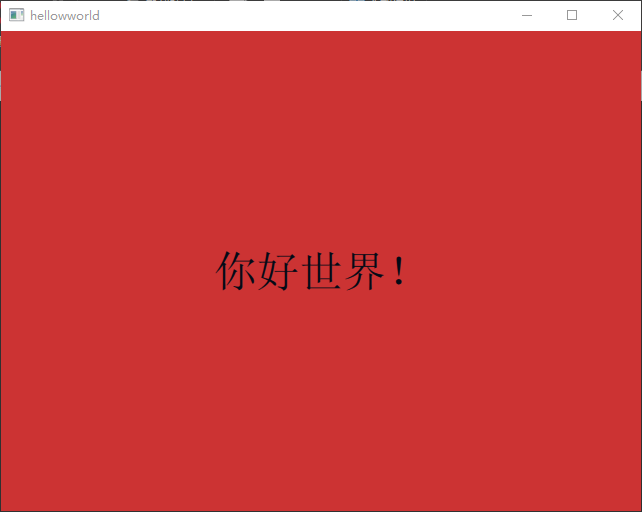
\includegraphics[width=0.95\textwidth]{../chapter01/hellowworld/the_app.png} %图片路径
\caption{你好世界!} %标题
\label{p000006} %索引
\end{figure}
%end图片


绝大多数介绍计算机语言的书籍都有一
个“Hellow World!”的案例,本书也不能免俗。

本章的C{\sourcefonttwo{}+}{\sourcefonttwo{}+}代码
如\lstlistingname\ \ref{f000030}:

%\begin{spacing}{1.0}
\FloatBarrier
\begin{lstlisting}[escapeinside={(*@}{@*)},
label=f000030,
caption=GoodLuck,
title=\lstlistingname\ \thelstlisting
]
#include <sstd_qt_and_qml_library.hpp>

int main(int argc, char ** argv) {

    /*初始化程序*/
    auto varApp = sstd_make_unique< sstd::Application >(argc, argv);
    /*初始化Qml/Quick引擎*/
    auto varWindow = sstd_make_unique< sstd::DefaultRoowWindow >();
    {
        /*获得Qml文件绝对路径*/
        auto varFullFileName = sstd::getLocalFileFullPath(
            QStringLiteral("myqml/hellowworld/main.qml"));
        /*加载Qml文件*/
        varWindow->load(varFullFileName);
        /*检查并报错*/
        if (varWindow->status() != sstd::LoadState::Ready) {
            qWarning() <<
                       QStringLiteral("can not load : ")
                       << varFullFileName;
            return -1;
        }
    }
    varWindow->show();

    return varApp->exec();

}(*@\marginpar[\hfill\fbox{\footnotesize{\lstlistingname\ \thelstlisting}}]{\fbox{\footnotesize{\lstlistingname\ \thelstlisting}}}@*)\end{lstlisting}          %抄录环境
%\end{spacing}
%main.cpp

本书将大量的程序细节隐藏到了“sstd\underline{\hspace{0.5em}}qt\underline{\hspace{0.5em}}and\underline{\hspace{0.5em}}qml\underline{\hspace{0.5em}}library”库里面。

\begin{itemize}
\item sstd::Application用于构造QApplication,
并初始化Qt Quick运行所需的参数;
\item sstd::DefaultRoowWindow在Debug
模式下继承自QQuickWidget,在Release模式下继承自QQuickView;
\item sstd::getLocalFileFullPath在
Debug模式以当前文件目录作为根目录,在Release模式下以应用程序
目录作为根目录;
\end{itemize}

本书以后章节的“main.cpp”都大同小异,以后不再赘述。


“main.qml”如\lstlistingname\ \ref{f000031}
所示:

%\begin{spacing}{1.0}
\FloatBarrier
\begin{lstlisting}[escapeinside={(*@}{@*)},
label=f000031,
caption=GoodLuck,
title=\lstlistingname\ \thelstlisting
]
/*main.qml*/
import QtQuick 2.9
import "main_private" as MainPrivate

Rectangle {

    width: 640
    height: 480
    color: Qt.rgba(0.8, 0.8, 0.8, 1)

    MainPrivate.MainText {
        z: 1
        anchors.fill: parent
    } /*~MainText*/

    MainPrivate.MainRectangle {
        z: 0
        anchors.fill: parent
    } /*~MainRectangle*/
} /*~Rectangle*/(*@\marginpar[\hfill\fbox{\footnotesize{\lstlistingname\ \thelstlisting}}]{\fbox{\footnotesize{\lstlistingname\ \thelstlisting}}}@*)\end{lstlisting}          %抄录环境
%\end{spacing}
%main.qml

\begin{itemize}

\item 第3行展示了如何引入其他目录的Qml文件。
其语法如\lstlistingname\ \ref{f000034}
所示:

%\begin{spacing}{1.0}
\FloatBarrier
\begin{lstlisting}[escapeinside={(*@}{@*)},
label=f000034,
caption=GoodLuck,
title=\lstlistingname\ \thelstlisting
]
import "ResourceURL" as Qualifier(*@\marginpar[\hfill\fbox{\footnotesize{\lstlistingname\ \thelstlisting}}]{\fbox{\footnotesize{\lstlistingname\ \thelstlisting}}}@*)\end{lstlisting}          %抄录环境
%\end{spacing}
%1.txt

\item 第5行定义了一个Rectangle:

%%%%%%%%%%%%%%%%%%%%%%%%%%%%%%%%%%%%%%%%%%%%%%%%%%

\begin{itemize}
\item 第7行定义了Rectangle的宽度;
\item 第8行定义了Rectangle的高度;
\item 第9行定义了Rectangle的颜色;
\end{itemize}

\item 第11\raisebox{0.16ex}{\sourcefonttwo\~{}}19行定义了两个子对象。
和Qt Widgets一样,子对象在父对象之上。兄弟对象之间的关系是,
后出现的对象在先出现的对象之上。
也可以调整z属性调整兄弟对象的上下关系。

读者可以尝试注释掉第12行和17行观察程序输出结果。

%%%%%%%%%%%%%%%%%%%%%%%%%%%%%%%%%%%%%%%%%%%%%%%%%%

\item 第13行和第18行使用“anchors”确保子对象完全覆盖父对象。

\end{itemize}

“MainRectangle.qml”如\lstlistingname\ \ref{f000032}
所示:
%\begin{spacing}{1.0}
\FloatBarrier
\begin{lstlisting}[escapeinside={(*@}{@*)},
label=f000032,
caption=GoodLuck,
title=\lstlistingname\ \thelstlisting
]
/*main_private/MainRectangle.qml*/
import QtQuick 2.9

Rectangle {
    color: Qt.rgba(0.8, 0.2, 0.2, 1)
}(*@\marginpar[\hfill\fbox{\footnotesize{\lstlistingname\ \thelstlisting}}]{\fbox{\footnotesize{\lstlistingname\ \thelstlisting}}}@*)\end{lstlisting}          %抄录环境
%\end{spacing}
%MainRectangle.qml

Qml是一门大小写敏感的计算机语言。
读者使用import命令引入Qml定义的对象时,文件名必须以大写开头;
而引入JavaScript文件时,
文件名应当以小写开头。

“MainText.qml”如\lstlistingname\ \ref{f000033}
所示:

%\begin{spacing}{1.0}
\FloatBarrier
\begin{lstlisting}[escapeinside={(*@}{@*)},
label=f000033,
caption=GoodLuck,
title=\lstlistingname\ \thelstlisting
]
/*main_private/MainText.qml*/
import QtQuick 2.9

Text {
    text: qsTr("你好世界!")
    color: Qt.rgba(Math.random() / 10, Math.random() / 10,
                   Math.random() / 10, 1)
    font.pointSize: 32
    verticalAlignment: Text.AlignVCenter
    horizontalAlignment: Text.AlignHCenter
}(*@\marginpar[\hfill\fbox{\footnotesize{\lstlistingname\ \thelstlisting}}]{\fbox{\footnotesize{\lstlistingname\ \thelstlisting}}}@*)\end{lstlisting}          %抄录环境
%\end{spacing}
%MainText.qml

\begin{itemize}

\item 第5行展示了如何在Qml中实现国际化,读者只需要用
qsTr包装字符串即可;
\item 第6\raisebox{0.16ex}{\sourcefonttwo\~{}}7行展示了可以在Qml中直接使用JavaScript;


\end{itemize}










%使用xelatex编译
%版权所有,翻版必究
%本文件由程序自动生成,任何修改将被覆盖
%2019 年 01 月 09 日



